\section{Project Statement}\label{sec:problem}

A CubeSat is a small satellite ($\sim$~1kg) constructed out of (usually)
commodity components that is used for scientific research or educational
purposes.  The University of Illinois has a
CubeSat\footnote{\url{http://cubesat.ae.illinois.edu/index.php}} program in
which a class and dedicated team have been developing a scalable picosatellite
bus, IlliniSat-2 (hereafter referred to as ``IlliniSat.''  IlliniSat is intended
to be used for multiple missions, the first of which (Lower
Atmosphere/Ionosphere Coupling Experiment, LAICE) is planned to launch around
December 2014.  This mission will involve three scientific payloads: one from
Illinois and two from Virginia Tech.  In collaboration with Bindu Jagannatha and
Alex Ghosh of the IlliniSat team, this project aims to analyze and enhance the
reliability of the computing systems used in IlliniSat.

The IlliniSat bus contains various systems, and this project focuses on the
Command and Data Handling (C\&DH) system.  The C\&DH system is responsible for
maintaining the mission schedule and coordinating the communication of the
satellite with the ground station.  It also interacts with other systems, such
as the Attitude Determination and Control System (ADCS), which is responsible
for maintaining proper orientation of the satellite. A state diagram for
IlliniSat, provided by the IlliniSat team, is shown in Figure
\ref{fig:state_machine}. The C\&DH system is based on a MitySOM-335x Processor
Card, built with a TI AM335x Application Processor System-on-Chip
(SoC).\footnote{\url{http://www.criticallink.com/wp-content/uploads/MitySOM-335x_Datasheet.pdf}}
An embedded Linux distribution, Arago, is run on top of the TI SoC and
IlliniSat's functionality is implemented in set of userspace daemons. The
standard \fix{atd} utility (modified for the IlliniSat platform) is used to
schedule tasks.

%FIXME: increase font size?
\begin{figure}
  \centering
  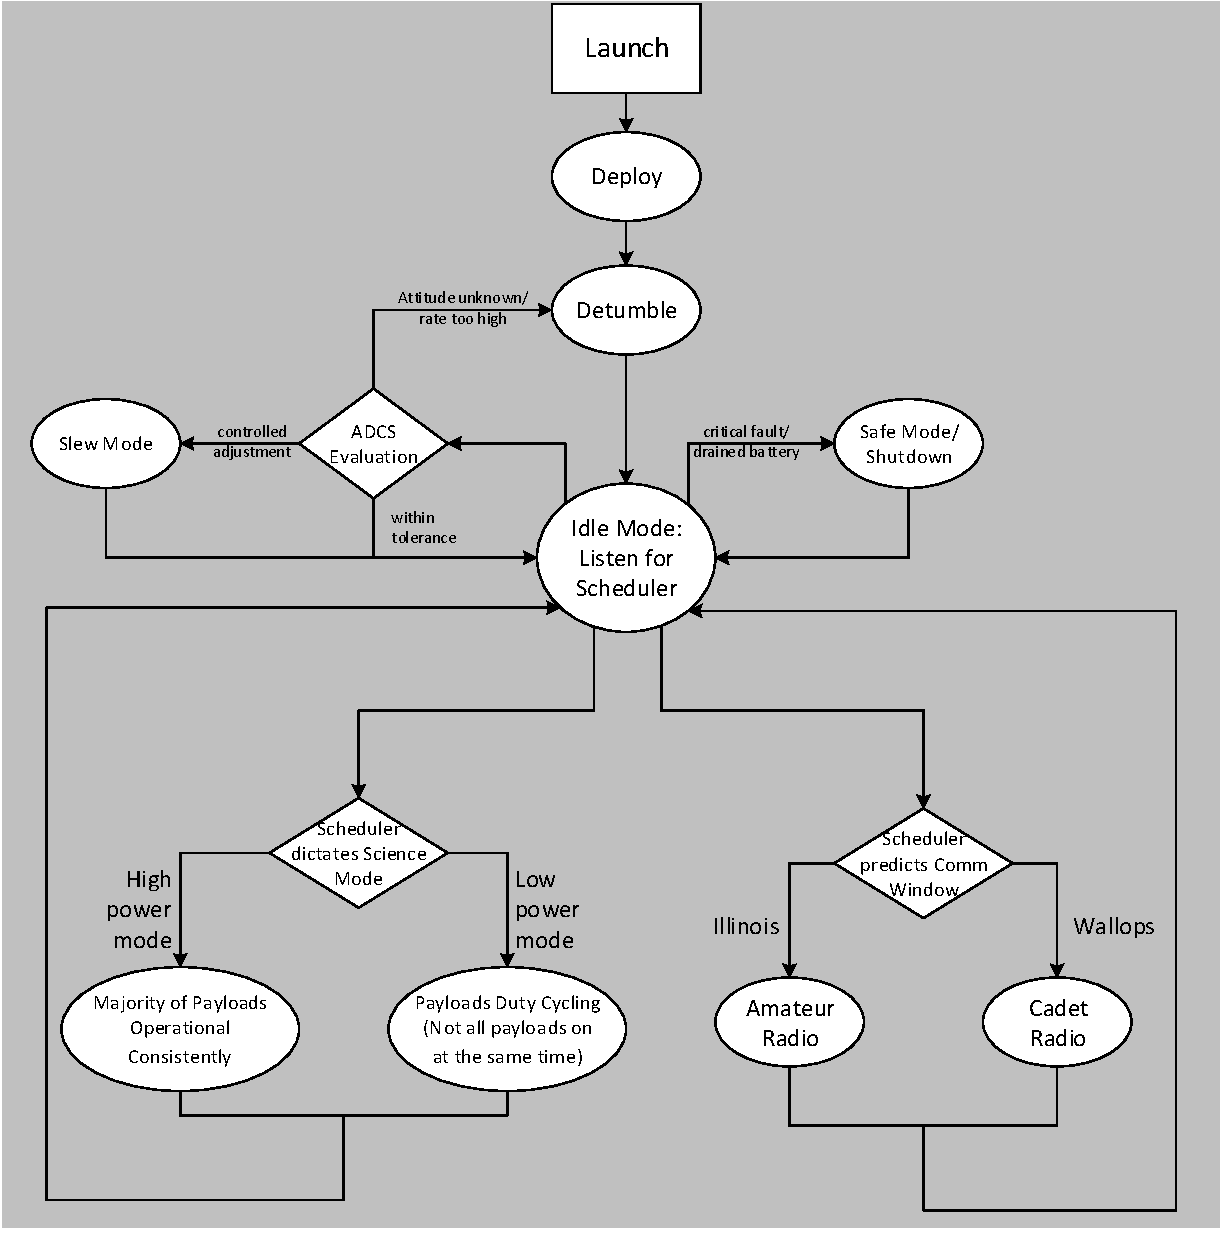
\includegraphics[width=0.5\textwidth]{images/state_machine}
  \caption{State diagram for IlliniSat-2, courtesy Alex Ghosh and Bindu
  Jagannatha. The main function of the C\&DH system is to operate the satellite
  through this state diagram. After launch and deploy, the system starts in the
  detumble state (which can also be reentered in an emergency situation): it
  calculates its attitude and points to the sun to charge the battery.  Idle:
  this is the mode where the satellite works through its mission schedule and
  ensures it has the proper attitude for data collection, the system can remain
  in this state to charge its battery.  Science modes: this is the normal
  operating mode of the satellite where the C\&DH subsystem collects data, and
  if there is not enough power it will only run a subset of the experiments.
  Communication modes: this is when a radio is active and communicating with a
  ground station. Slew mode: C\&DH relinquishes control to the ADCS when it
  detects that the satellite may need repositioning.  Safe mode: low-power
  default mode when a fault is detected, the satellite will broadcast an error
  code to the ground station.  Shutdown: all non-crucial systems are shutdown
  when battery power is critically low.  }\label{fig:state_machine}
  %FIXME: finish writing this
\end{figure}

Currently, the system has a watchdog timer that will reboot the flight computer
if it does not receive a heartbeat every 60 seconds.  The watchdog is part of a
health monitoring system that also observes the state of the battery, satellite
attitude, temperature, etc. If the health monitor determines that the system is
in a faulty state, it will transition C\&DH into a recovery mode (e.g. if the
battery is low, switch off all nonessentials and point the satellite towards the
sun).
%FIXME: do we want the health monitor figure?
%FIXME: define SPoF

\subsection{Design Constraints}
The IlliniSat bus has many hardware and software requirements that constrain our
improvements of the system. Since the IlliniSat team has already chosen their
hardware, we will have to make all of our changes in software. Given the nature
of the mission, the software is required to have mission critical components
that cannot fail. The main design constraints that will be put on us while
improving the system are the following:
\begin{itemize}
  \item Preserve real-time deadlines
  \item Minimize additional power consumption
  \item Avoid complex solutions
\end{itemize}
IlliniSat needs to be constantly reacting to its environment so that it can
interface with payloads, communicate to the ground, and monitor the health of
the system, among other things. Because of this, hard real-time deadlines are
required and cannot be missed. 

Since IlliniSat is such a small satellite with stringent physical dimensions and
therefore limited battery capacity, power is a major concern for the team.  If
too much power is consumed, the battery may not last while the satellite is not
receiving solar power (if it is either eclipsed by the earth or positioned
poorly).  Also, if the system is charging and the CPU is loaded, components may
start to overheat.  Any software reliability techniques used should therefore be
mindful not to use too much power and should also be aware of the current state
of the satellite (recovery modes, etc...).

Finally, the IlliniSat team has requested that we keep our solution simple (and
well documented) so that it can be implemented and maintained easily.
Furthermore, we need to be careful not to implement overly intricate solutions
that may introduce new failure modes or reduce the system's reliability.
